
%----------------------------------------------------------------------------------------
%	PACKAGES AND OTHER DOCUMENT CONFIGURATIONS
%----------------------------------------------------------------------------------------

\documentclass[12pt]{article}
\usepackage[english]{babel}
\usepackage{amsmath}
\usepackage{graphicx}
\usepackage{float}
\usepackage[colorlinks = true,
linkcolor = blue,
urlcolor  = blue,
citecolor = blue,
anchorcolor = blue]{hyperref}
\usepackage{blindtext}


\begin{document}
	
	\begin{titlepage}
		
		\newcommand{\HRule}{\rule{\linewidth}{0.5mm}} 
		
		\center % Center everything on the page
		
		%----------------------------------------------------------------------------------------
		%	HEADING SECTIONS
		%----------------------------------------------------------------------------------------
		\textsc{\Large MSc Project: Mobile Hairdresser Application}\\[5 cm] 

		
		
		
\includegraphics[scale=0.05]{images/logo.png}\\[1 cm]
				
		

		
		
		\textsc{\LARGE Joshua Robertson} \\[6 cm]
		
		

		
		
		%----------------------------------------------------------------------------------------
		%	TITLE SECTION
		%----------------------------------------------------------------------------------------
		
		
		
		%----------------------------------------------------------------------------------------
		%	AUTHOR SECTION
		%----------------------------------------------------------------------------------------
		
		
		\begin{center}
			
			\textsc\emph{{“A dissertation submitted to the University of Bristol in accordance with the requirements of the degree of Master of Science by advanced study in Computer Science in the Faculty of Engineering."}} \\[1.2 cm]
			
			School of Computer Science, Electrical and Electronic Engineering, and Engineering Maths (SCEEM) \\[1 cm]
			
			
			
		\end{center}
		
		
		
		
		\vfill % Fill the rest of the page with whitespace
		
	\end{titlepage}
	
	\section{Introduction}
	The COVID pandemic has brought with it a shift in perceptions around leaving the home and with that a desire for more homeworking and access to remote services. For example, remote workers show an increase in job satisfaction \cite{flexjobs, 2019}, \cite{CNBC, 2020}, are more productive, have better mental health \cite(flexjobs, 2020) and even make more money (ADD CITE).
	
	New Product Development refers to the entirety of processes leading to bringing a product to market and encompasses several steps as seen in figure \ref{fig:npd} below.
	\newline
	
	\begin{figure}[H]
		\centering
		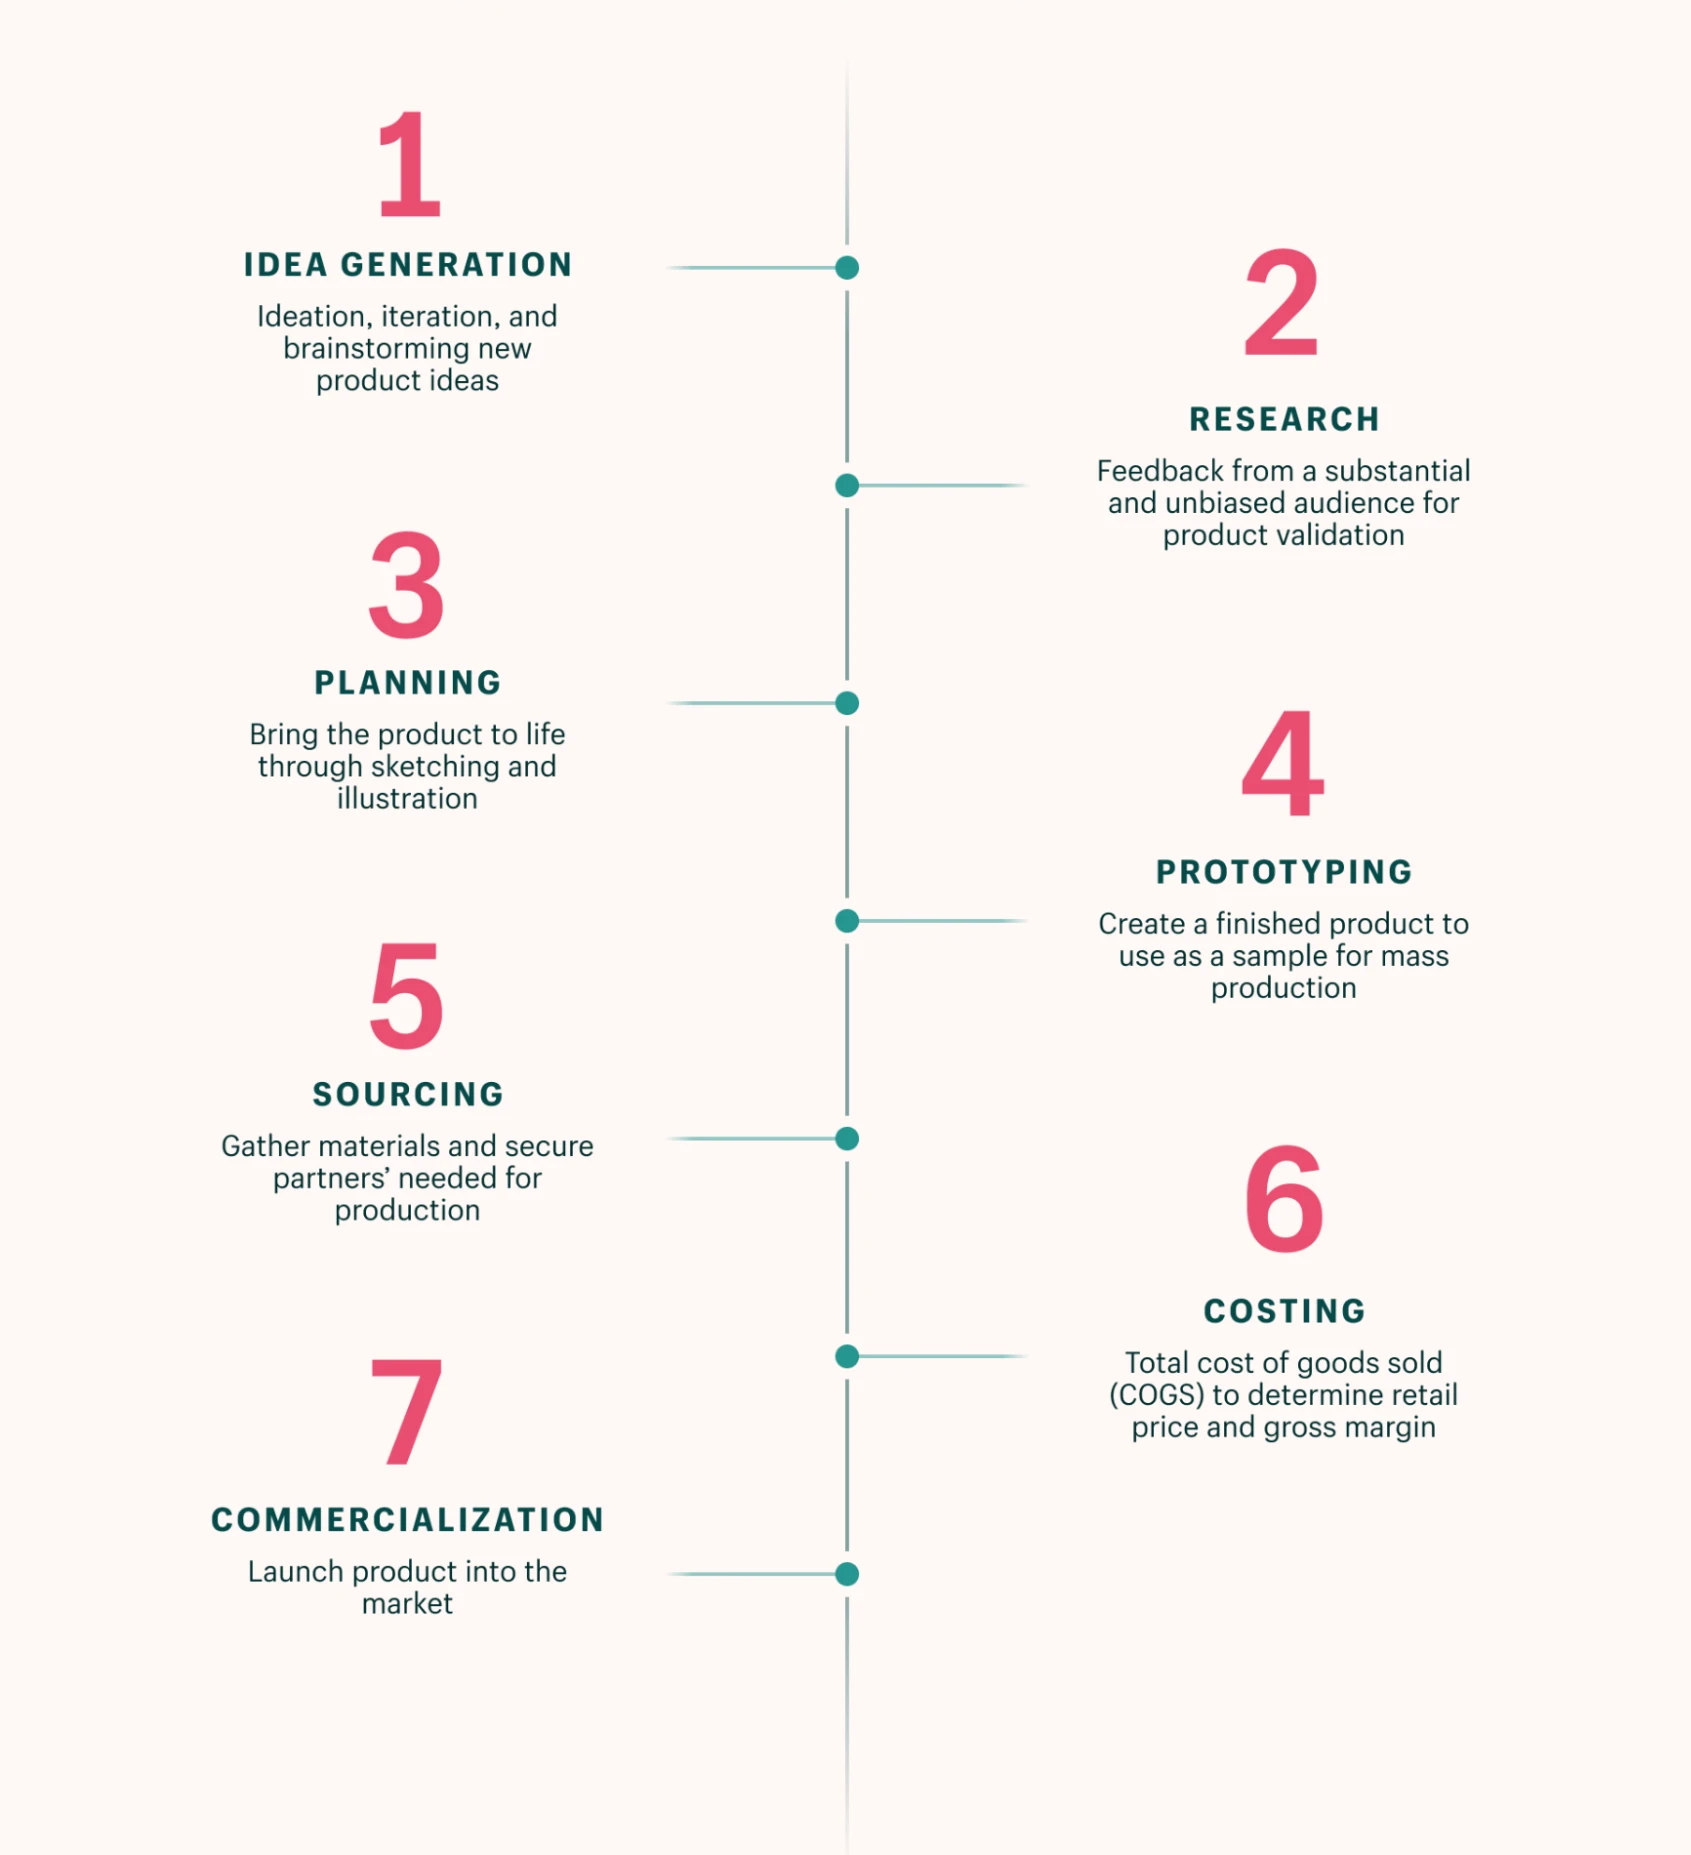
\includegraphics[scale=0.15]{images/npd.png}
		\caption{The 7 Steps of New Product Development}
		\label{fig:npd} \cite{shopify}
	\end{figure}
	
	
	\subsection{Ideation and Concept}
	\blindtext
	
	\subsection{Market Analysis}
	In order to gauge whether there is a market for the proposed analysis, a survey was carried out in which users were asked about whether they could see themselves using the application features, among other things.
	 
	\subsubsection{Existing Applications}
	
	
	\subsubsection{The Target User}
	
	\subsubsection{Programming Language}
	When deciding on the programming software, several metrics were taken into consideration, including cross-platform functionality, speed, speed of development and performance. For this reason, Dart and the corresponding Flutter software development kit (SDK) were chosen for the primary software. Flutter is a cross-platform development kit, meaning that it will natively run on both iOS and android applications created by Google \cite{flutter}. Dart is compiled ahead-of-time into native ARM code giving better performance compared to other similar development kits, such as React Native and the user interface  is implemented within a fast, low-level C++ library giving great speed to the application. Dart has also seen a large increase in usage within recent years, jumping up 532\% from 2018 to 2019 \cite{Github, 2018} meaning that there is now an extensible list of third-party plugins available and a large community.
	

	\subsection{User Personas}
	The creation of user personas representing fictitious, archetypal users is an essential part of application development \cite{Grudin and Pruitt, 2002} and allows a deep understanding of the target user to be sought and implemented within the features and design of the application \cite{Long, 2009}. Although there are some shortcomings to qualitative persona generation, such as validity concerns and user bias \cite{Chapman and Milham, 2007} which are addressed by other methods, such as data-driven personas \cite{Mcginn and Kotamraju, 2008}, we have decided to stick with qualitative methods, which allow for enough brevity and depth for the scope of the project. Here we created 3 personas, which are discussed in detail below.
	\begin{itemize}
		\item Persona 1: 
		
		INSERT PERSONA INFO
		\item Persona 2:
		\item Persona 3:
	\end{itemize}


	\subsection{Sprints}
	\subsubsection{Sprint 1 - Setup}
	During the first sprint, the task involved setting up the environment in preparation to begin development. For the editor, Android Studio was 

	
\end{document}